\section{Design Methodologies}
\paragraph{}
One approach for VLSI Design is using a cost function with the required factors as the inputs of the function. The General form of the cost function can be show as (\textbf{i} is a component):\[
	\mathbf{C}\,=\,\sum_{i\,=\,1}^{N}\left(\,w_{p}\\,P_{1}\,+\,w_{D}\,\frac{L_{i}}{V_{i}(t)}+w_{A}\,A_{i}\right)
\]
Where \large{\(\mathit{C}\)} is the\textbf{ cost function} and; {\large\(P_{i}\)} is the \textbf{Power Consumption} \newline
of \textbf{component i}; \large{\(\mathit{L_{i}}\)} is length of the path for the \(i\);
\large{\(V_{i}(t)\)} is the voltage of \(i\) at time \(t\); \large{\(\mathit{A_{i}}\)} is the Area of \(i\) and, \large{\(w\)} is the weight of each factor relevant to its importance (in this simplified formula \(p\) is for power, \(D\) for delay and, \(A\) for area).\newline
Designing a cost function usually tends to become more complex and time consuming as the factors grow.\\ Thereby a proper approach is necessary to reduce the complexity, this can be achieved through \textbf{Divide and Conquer} methodology by breaking down a large chip into smaller parts and abstract away the unnecessary details of the blocks \autoref{abs_main}.
\begin{figure}[b!]  
\usetikzlibrary {through}
\tikzset{auto}

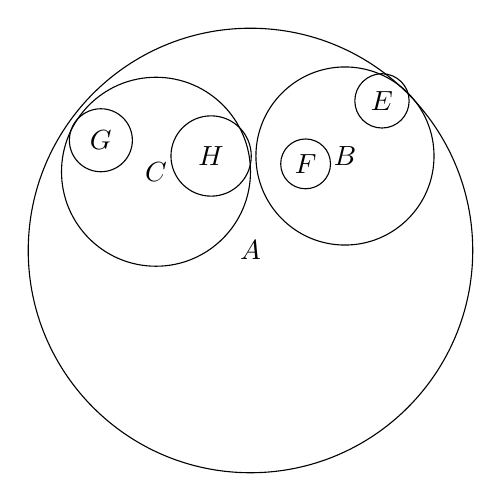
\begin{tikzpicture}
	
	\node [draw] at (0,0) [circle through={(2,2)}] {$A$};
	\node [draw] at (1.2,1.2) [circle through={(2,2)}] {\(B\)};
	\node [draw] at (1.67,1.9) [circle through={(2,2)}] {\(E\)};
	\node [draw] at (0.7,1.1) [circle through={(1,1)}] {\(F\)};
	\node [draw] at (-1.2,1) [circle through={(0,1)}] {\(C\)};
\node [draw] at (-1.9,1.4) [circle through={(-1.9,1)}] {\(G\)};
\node [draw] at (-0.5,1.2) [circle through={(0,1.1)}] {\(H\)};
\end{tikzpicture}
\hspace{4em}
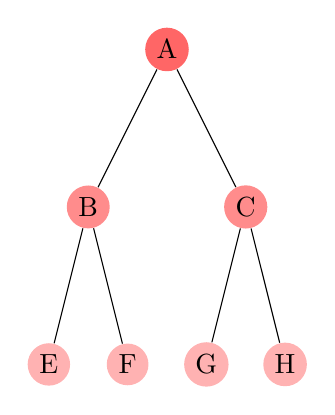
\begin{tikzpicture}
	[level distance=20mm,
	every node/.style={fill=red!60,circle,inner sep=2pt},
	level 1/.style={sibling distance=20mm,nodes={fill=red!45}},
	level 2/.style={sibling distance=10mm,nodes={fill=red!30}},
	level 3/.style={sibling distance=5mm,nodes={fill=red!25}}],
	\
	\node {A}
	child {node {B}
		child {node {E}}
		child {node {F}}
	}
	child {node {C}
		child {node {G}}			
		child {node {H}}
	};

\end{tikzpicture}
\caption{design hierarchy examples}
\label{abs_main}
\end{figure}